\section{Komparatoren / Schmitt-Trigger}

\begin{itemize}
    \item OpAmp-Ausgang meistens am Anschlag $V_{\rm out_{max}}$ bzw. $V_{\rm out_{min}}$
    \item Rückkopplungsfrei oder Rückkopplung auf \textbf{positiven} Eingang
\end{itemize}

\vspace{0.2cm}

Schmitt-Trigger werden verwendet, wenn Signale \textbf{verrauscht} sind oder zur \textbf{Störungsunterdrückung} auf CLK-Signalen.


\subsection{OPV als Komparator}

\begin{minipage}[c]{0.4\columnwidth}
    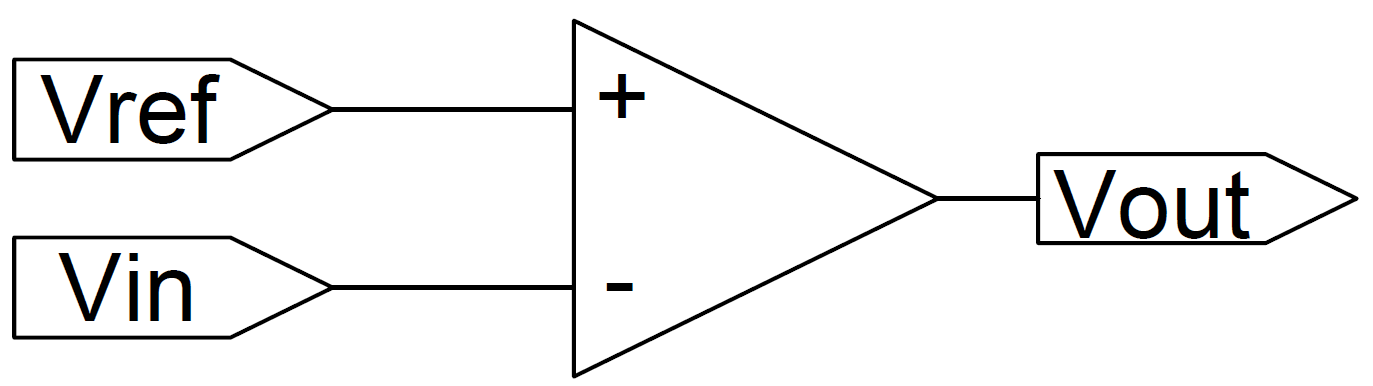
\includegraphics[width=\columnwidth]{images/komparator.png}
\end{minipage}
\hfill
\begin{minipage}[c]{0.48\columnwidth}
    Vergleicht $V_{\rm opp}$ mit $V_{\rm opn}$ bzw.$ V_{\rm ref}$ mit $V_{\rm in}$
\end{minipage}

\vspace{0.2cm}

\begin{itemize}
    \item Nur in sehr kleinem Bereich ist OpAmp in linearem Bereich
    \item Jeder OpAmp kann als Komparator eingesetzt werden
    \item Es gibt Komparatoren als spezialisierte Bausteile
    \item Komparatoren dürfen \textbf{nicht} als OpAmps eingesetzt werden
\end{itemize}


\subsection{Vergleich OpAmp - Komparator}

\begin{center}
    \scalebox{0.9}{
    \begin{tabular}{@{}lll@{}}
        \toprule
        \textbf{Parameter / Eigenschaft}        & \textbf{Operationsverstärker}     & \textbf{Komparator}                       \\
        \midrule
        \textbf{Anstiegs- und Abfallzeit}       & mittel                            & klein                                     \\
        \midrule
        \textbf{Schaltverzögerung}              & mittel                            & klein                                     \\
        \midrule
        \textbf{Amplitudengang}                 & mittlere Bandbreite und Abfall    & hohe Bandbreite und Abfall                \\
                                                & mit $- 20 \deci \bel$ / Dekade    &  steiler as $- 20 \deci \bel$ / Dekade    \\

        \midrule
        \textbf{Slew Rate}                      & mittel                            & sehr gross                    \\
        \bottomrule
    \end{tabular}}
\end{center}

\vspace{0.1cm}

\begin{minipage}{0.48\columnwidth}
    
    \begin{center}
        \myul{\textbf{Komparator}}
        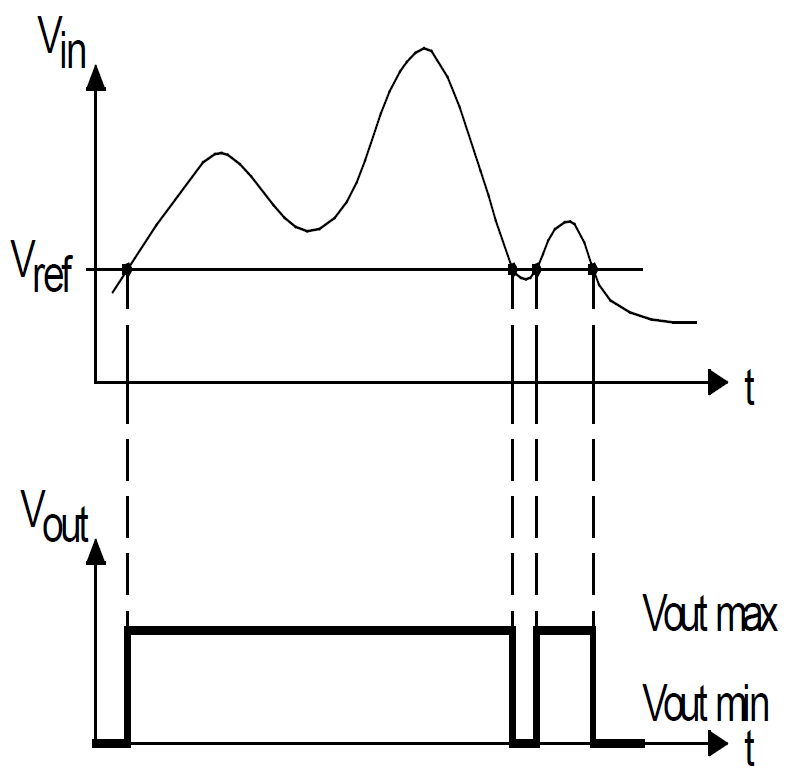
\includegraphics[width=0.75\columnwidth]{images/signalverlauf_komparator.png}
    \end{center}

    \begin{itemize}
        \item 1 Schaltschwelle
        \item Glitches möglich
    \end{itemize}
\end{minipage}
\hfill
\begin{minipage}{0.48\columnwidth}
    \begin{center}
        \myul{\textbf{Schmitt-Trigger}}
        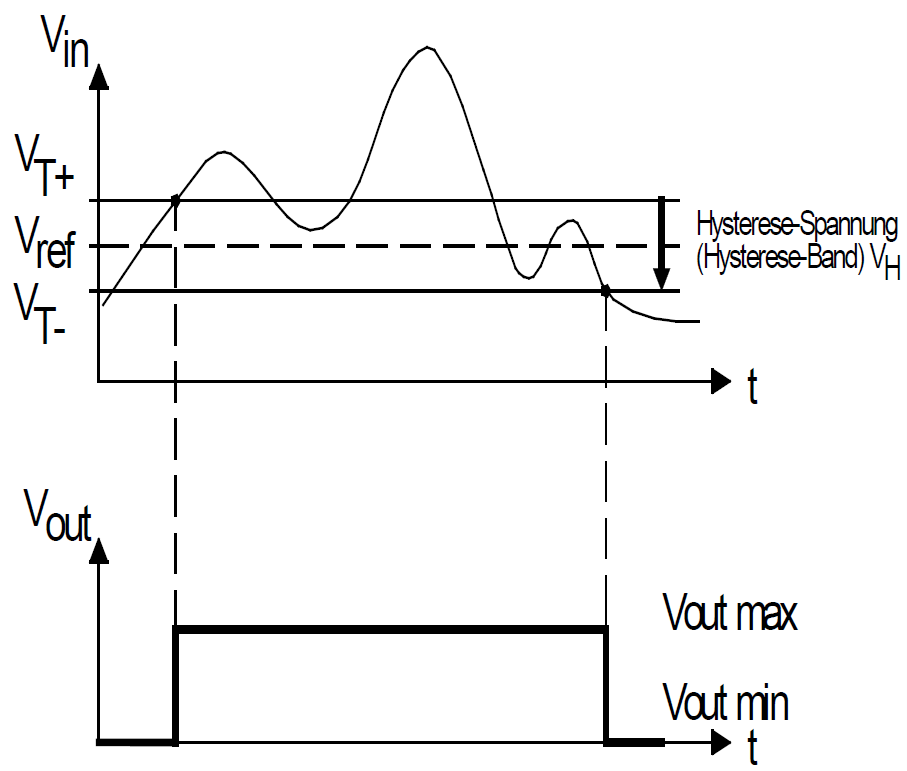
\includegraphics[width=0.8\columnwidth]{images/signalverlauf_schmitt-trigger.png}
    \end{center}

    \begin{itemize}
        \item 2 Schaltschwelle
        \item Glitches unterdrückt
        \item Hystere-Spannung $V_H$
    \end{itemize}
\end{minipage}


\subsection{Invertierender Schmitt-Trigger}

\begin{minipage}[c]{0.45\columnwidth}
    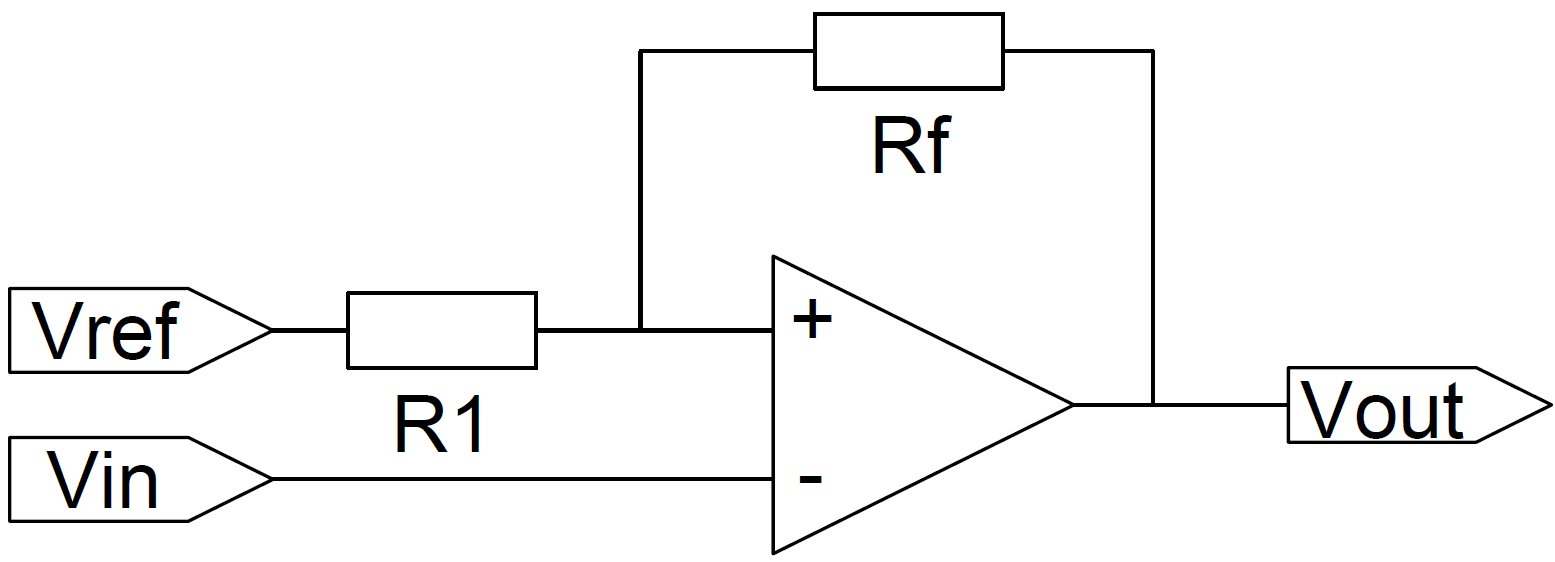
\includegraphics[width=\columnwidth]{images/invertierender_schmitt-trigger.png} 

    \vspace{0.1cm}

    Schaltet, wenn $V_{\rm in} = V_{\rm opp}$
\end{minipage}
\hfill
\begin{minipage}[c]{0.51\columnwidth}
    \begin{center}
        \myul{\textbf{Hysterese}}
        $$ \boxed{ V_H = V_{T-} - V_{T+} } $$
        $$ \boxed{ V_H = (V_{\rm out_{max}} - V_{\rm out_{min}} ) \frac{R_1}{R_1 + R_f} } $$
    \end{center}
\end{minipage}

\vspace{0.2cm}

$$ \boxed{ V_{\rm in} \text{-tief:} \quad V_{T+} = V_{\rm opp} = \frac{V_{\rm ref} \cdot R_f + V_{\rm out_{max}} \cdot R_1 }{R_1 + R_f} }  $$
$$ \boxed{ V_{\rm in} \text{-hoch:} \quad V_{T-} = V_{\rm opp} =  \frac{V_{\rm ref} \cdot R_f + V_{\rm out_{min}} \cdot R_1 }{R_1 + R_f} } $$


\subsection{Nicht-Invertierender Schmitt-Trigger}

\begin{minipage}[c]{0.45\columnwidth}
    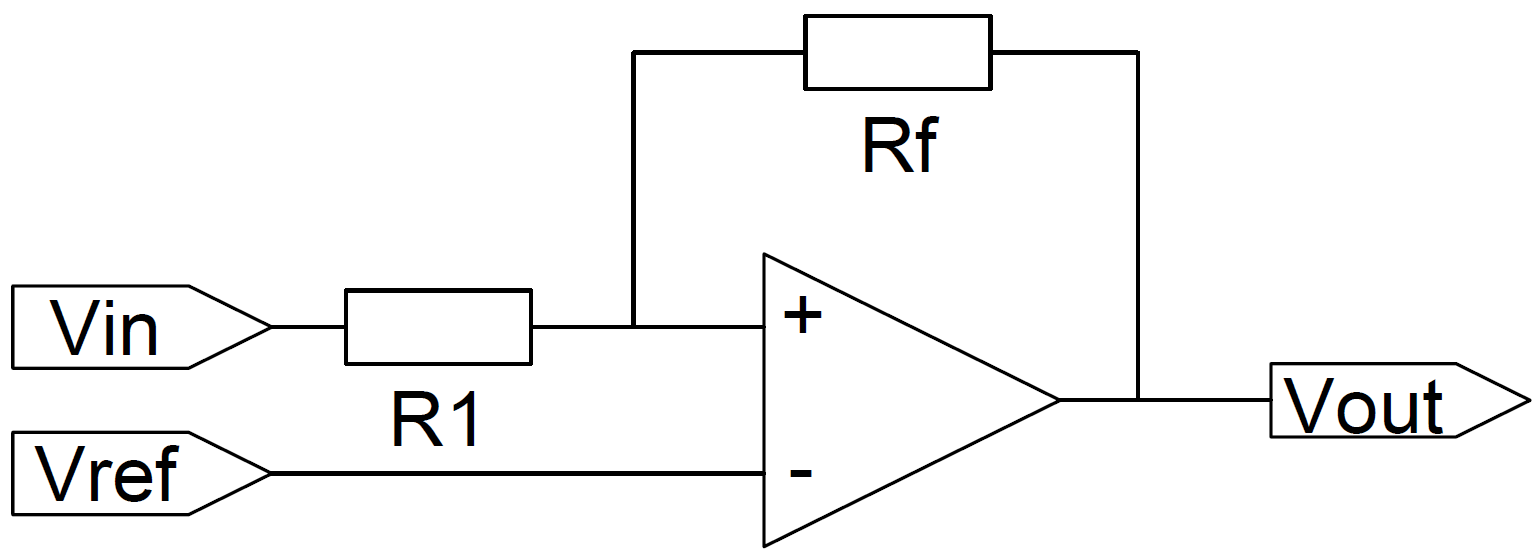
\includegraphics[width=\columnwidth]{images/nichtinvertierender_schmitt-trigger.png}

    \vspace{0.1cm}

    Schaltet, wenn $V_{\rm opp} = V_{\rm ref}$
\end{minipage}
\hfill
\begin{minipage}[c]{0.51\columnwidth}
    \begin{center}
        \myul{\textbf{Hysterese}}
        $$ \boxed{ V_H = V_{T+} - V_{T-} } $$
        $$ \boxed{ V_H = (V_{\rm out_{max}} - V_{\rm out_{min}} ) \frac{R_1}{R_f} } $$
    \end{center}
\end{minipage}


\begin{minipage}[t]{0.6\columnwidth}
    $$ \boxed{ V_{\rm in} \text{-hoch: } \quad V_{T-} = V_{\rm ref} \frac{R_1 + R_f}{R_f} - V_{\rm out_{max}} \frac{R_1}{R_f} }  $$
    $$ \boxed{ V_{\rm in} \text{-tief: } \quad V_{T+} = V_{\rm ref} \frac{R_1 + R_f}{R_f} - V_{\rm out_{min}} \frac{R_1}{R_f} } $$
\end{minipage}
\hfill
\begin{minipage}[t]{0.35\columnwidth}
    $$ \boxed{ V_{\rm opp} = \frac{  V_{\rm in} \cdot R_f + V_{\rm out} \cdot R_1}{R_1 + R_f} } $$
\end{minipage}

\vspace{0.2cm}

\textbf{Nachteil invertierender Schmitt-Trigger:} \\
'Kick-Back' auf Eingang wenn Ausgang schaltet

\vspace{0.2cm}

\textbf{Nachteil nicht-invertierender und invertierender Schmitt-Trigger:} \\
Hysterese und Schaltschwellen nicht unabhängig einstellbar


\subsection{Schmitt-Trigger mit frei wählbaren Schaltschwellen}

\begin{minipage}{0.38\columnwidth}
    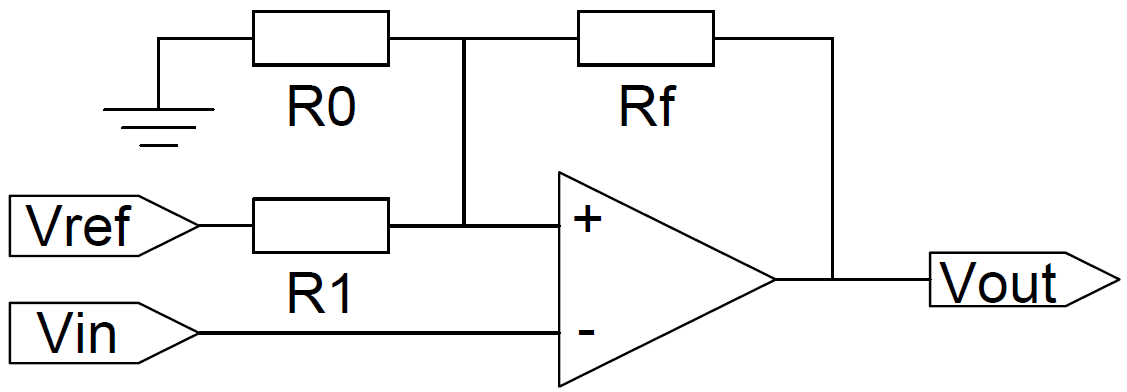
\includegraphics[width=\columnwidth]{images/inv_schmitt-trigger_schaltschwellen.png}
\end{minipage}
\hfill
\begin{minipage}{0.55\columnwidth}
    $$ \boxed{ V_{\rm opp} = V_{\rm ref} \, \frac{R_f || R_0}{R_1 + R_f || R_0} + V_{\rm out} \, \frac{R_1 || R_0}{R_1 || R_0 + R_f} } $$
\end{minipage}

\vspace{0.2cm}

2 Gleichungen, 3 Variablen ($R_0$, $R_1$, $R_f$) \\
\textrightarrow\ 1 Widerstand wird gewählt (z.B. $R_f = 100 \, \mathrm{k \Omega}$)

